\section{Streaming video using WebRTC}
Attempts were also made at integrating an example project from \gs  to stream videos using \gls{webrtc} \cite{gstreamerWebrtcMasterGStreamer2021}.
The example demonstrates the process of streaming video from a pipeline to a client within a web browser.
Given that a functional solution utilizingng \glspl{jpeg} had already been implemented, and considering the time-consuming nature of the integration task, it was not given high priority.
In future work acheiving this is probably the best approach as \gls{webrtc} has low latency compared to other protocols as depicted in Figure \ref{fig:streaming_latency} \cite{doughertyUltraLowLatency2022}.
\gls{webrtc} is built for low latency peer-to-peer communication over \gls{udp}, supports \gls{h265} encoding and will support \gls{av1} in the future \cite[1]{loretoRealTimeCommunicationWebRTC2014} \cite{ablyWebRTCVsWebSocket2023} \cite{mekyaFirstHEVC2652020}
\cite{red5proKeyReasonsAV12023}
\begin{figure}[H]
    \centering
    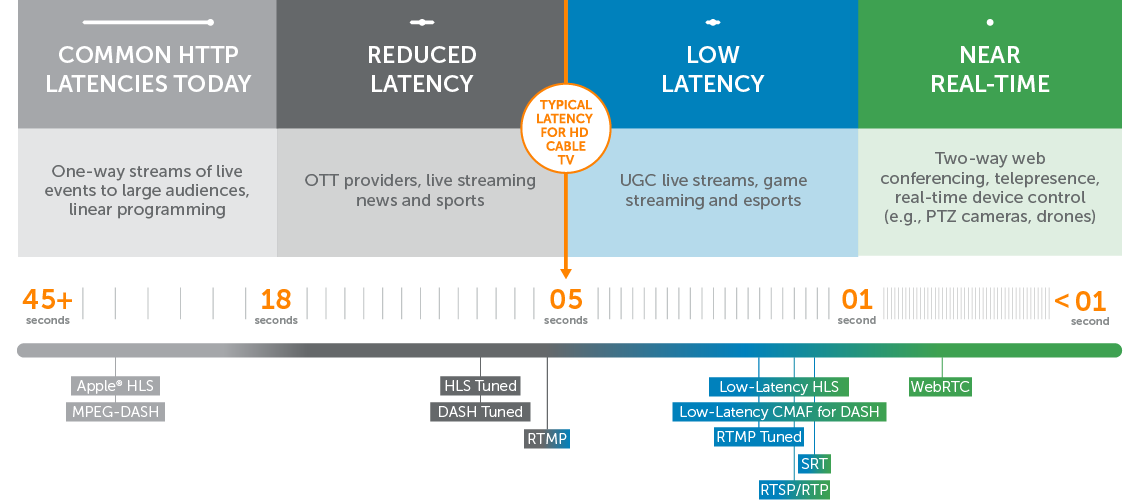
\includegraphics[width=\textwidth]{figures/webrtc_latency.png}
    \caption{Latency comparison of different streaming protocols \cite{doughertyUltraLowLatency2022}}
    \label{fig:streaming_latency}
\end{figure}